\section{Introduction}

% TODO
See the awesome Figure~\ref{110_map}.

Something about nonlinear dynamics in general and how discrete
nonlinear systems can display complexity with a small number of
parameters--e.g. logistic map.

\subsection{Elementary Cellular Automata}
% TODO

An Elementary Cellular Automaton (ECA) is defined in Stephen Wolfram's
\emph{A New Kind of Science}~\cite{anks}

\subsection{Automata Rules}
% TODO
- Rules and rule numbering

\subsection{Examples}
% TODO
- Examples (many figures)

% TODO
\begin{figure}
    \centering
    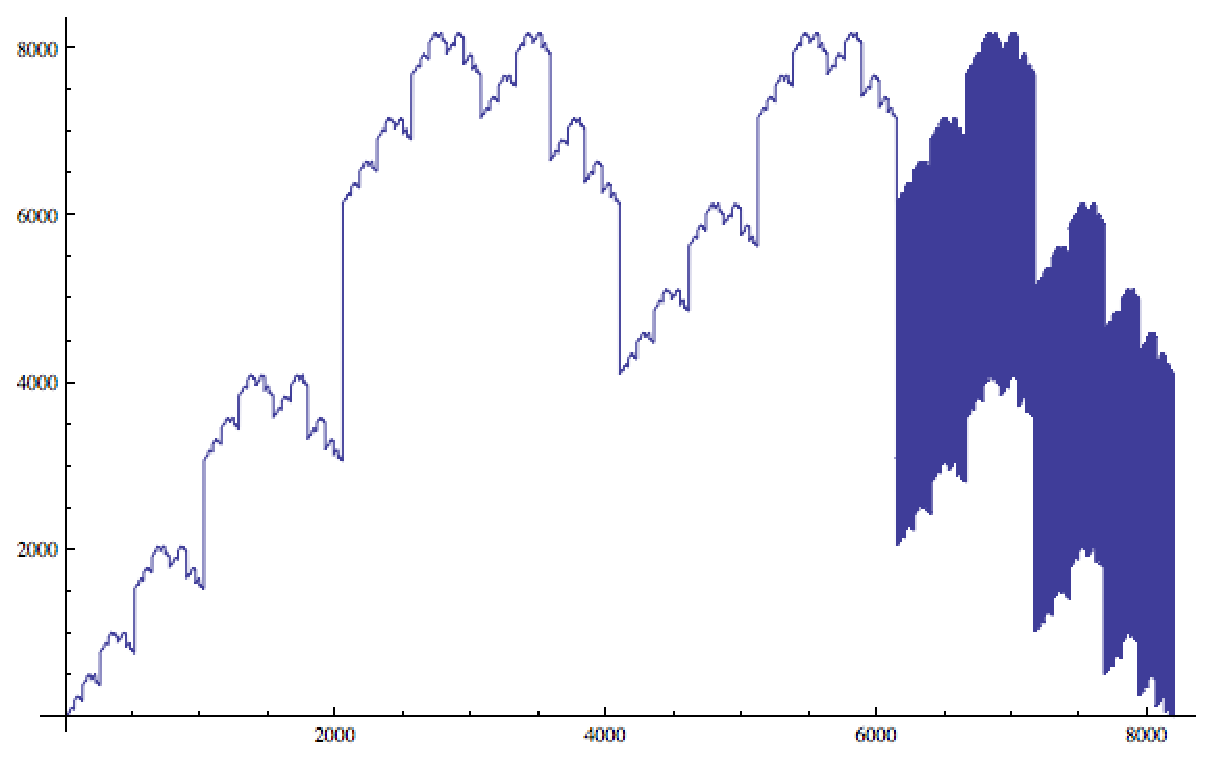
\includegraphics[width=0.49\textwidth]{110_13.eps}
    \caption{\label{110_map} Fractal map for rule 110 and a 13-site grid.}
\end{figure}

\begin{figure}
    \begin{minipage}[b]{0.49\textwidth}
        \centering
        
\includegraphics[width=\textwidth]{rule126.eps}
        \caption{\label{rule126} Rule 126}
    \end{minipage}
    \hspace{0.5cm}
    \begin{minipage}[b]{0.49\textwidth}
        \centering
        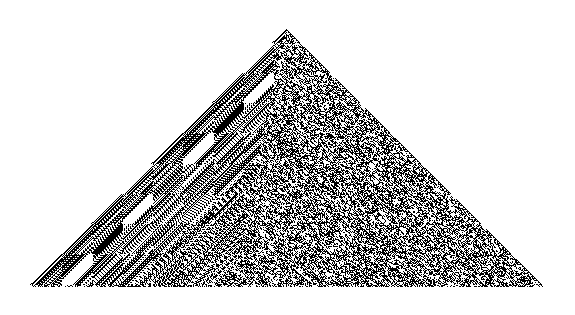
\includegraphics[width=\textwidth]{rule30.eps}
        \caption{\label{rule30} Rule 30}
    \end{minipage}
\end{figure}


\begin{figure}
    \begin{minipage}[b]{0.49\textwidth}
        \centering
        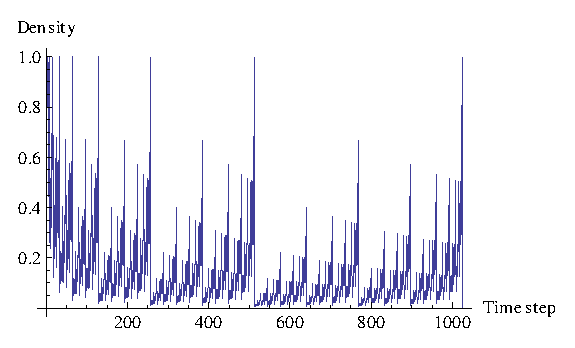
\includegraphics[width=\textwidth]{126density.eps}
        \caption{\label{126density} The Density of rule 126 plotted as a function of time step}
    \end{minipage}
    \hspace{0.5cm}
    \begin{minipage}[b]{0.49\textwidth}
        \centering
        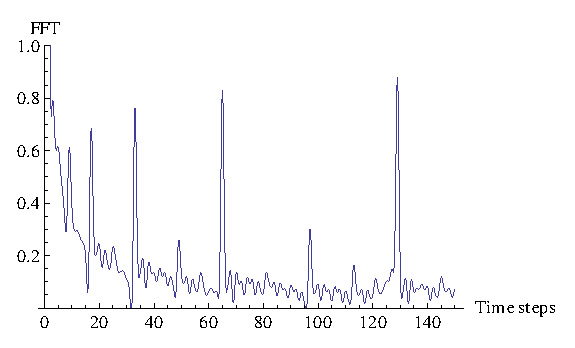
\includegraphics[width=\textwidth]{126FFT.eps}
        \caption{\label{126FFT} The FFT of rule 126's density, showing sharp peaks at 2$^n$.}
    \end{minipage}
\end{figure}


\begin{figure}
    \begin{minipage}[b]{0.49\textwidth}
        \centering
        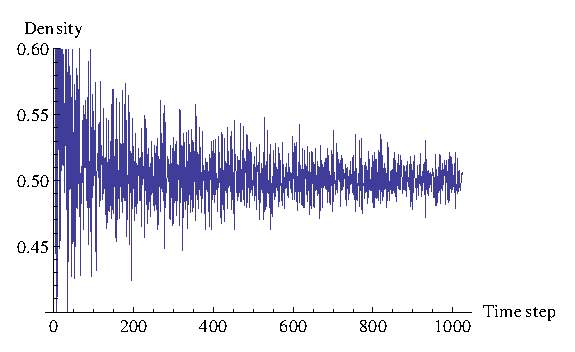
\includegraphics[width=\textwidth]{30density.eps}
        \caption{\label{30density} The Density of rule 30 plotted as a function of time step}
    \end{minipage}
    \hspace{0.5cm}
    \begin{minipage}[b]{0.49\textwidth}
        \centering
        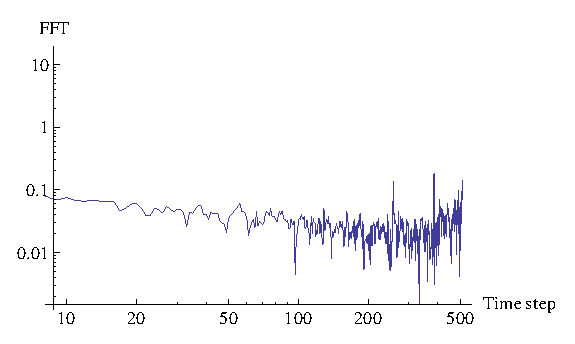
\includegraphics[width=\textwidth]{30FFT.eps}
        \caption{\label{30FFT} The FFT of rule 30's density.  The flat transform is the same as white noise.}
    \end{minipage}
\end{figure}
